\subsection{Survey screenshots}
  \subsubsection{Initial}
    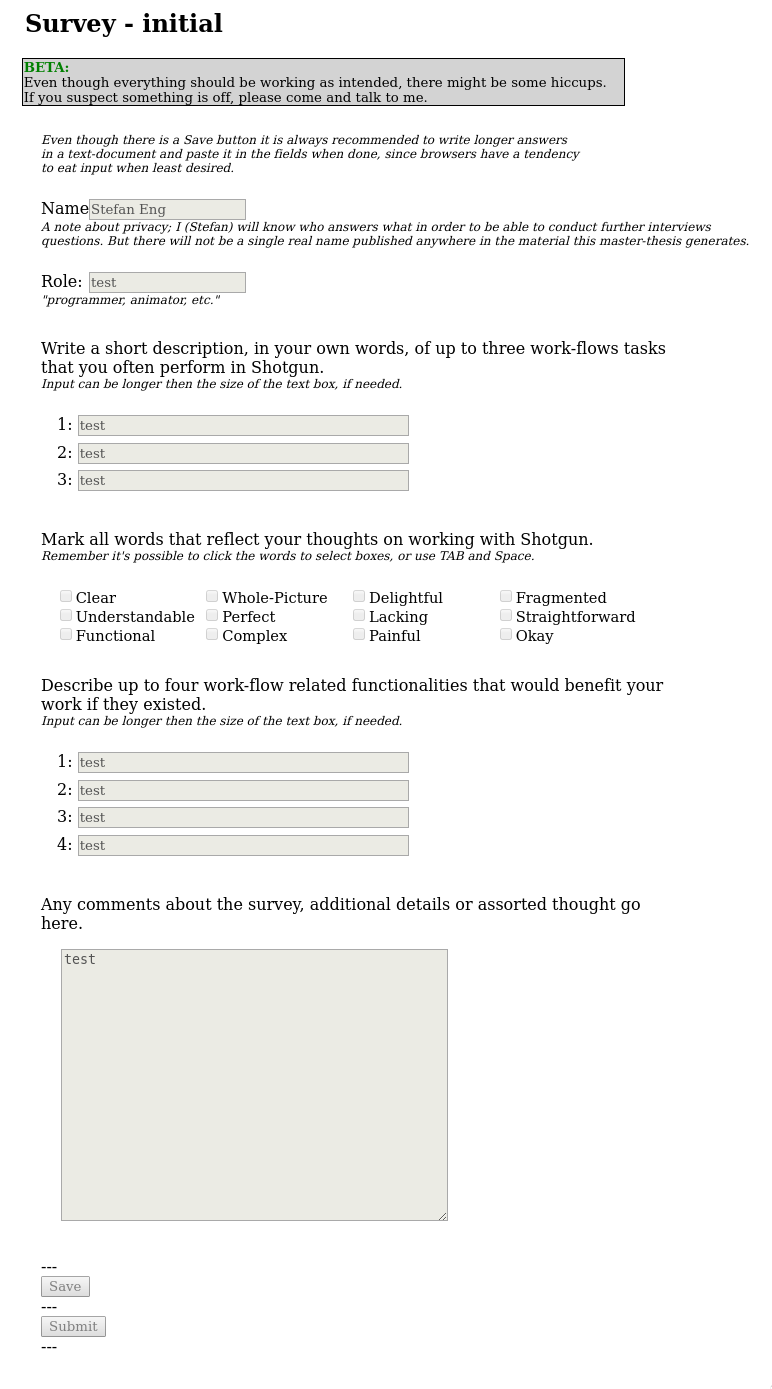
\includegraphics[width=\textwidth,trim={0cm 18cm 0cm 0cm},clip]{images/000_survey_initial.png}
    \newpage
    \begin{figure}[H]
      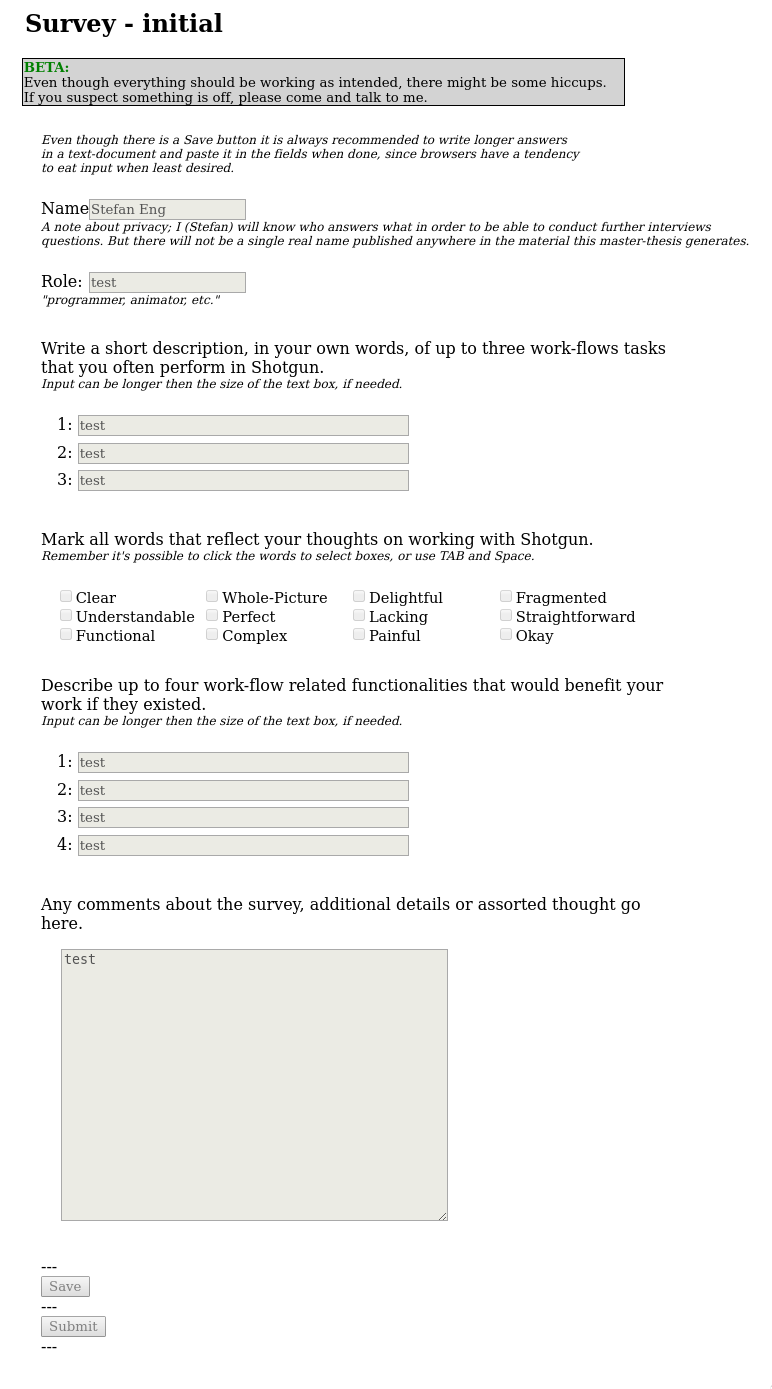
\includegraphics[width=\textwidth,trim={0cm 1cm 0cm 31cm},clip]{images/000_survey_initial.png}
      \caption{Screenshot of the initial survey.}
      \label{fig:ref_fig_survey_initial}
    \end{figure}

  \subsection{Survey data}
   \subsubsection{Initial}
      \label{subsec:ref_subsec_results_initial}
      \textbf{Q1: Write a short description, in your own words, of up to three
        work-flows tasks that you often perform in Shotgun:} \\
      \begin{adjustwidth}{0.3cm}{}
        Finding my tasks\\
        Time-logging on tasks\\
        Finding the right reference for a shot-task\\
        Upload Versions\\
        Find Tasks\\
        Gather Information\\
        find level camera\\
        find LD and ND names\\
        Find assest for scene\\
        follow priorities\\
        update tasks\\
        perform searches according different parameters\\
        task creation\\
        task follow up both towards director and artists\\
        task/artist feedback\\
        Change the status of a task\\
        log time on tasks\\
        search for prior versions on related tasks, to be able to complete current task\\
        Check work load for tech animators\\
        Check status of scenes or models\\
        Assign rigging and skinning tasks\\
        Update tasks with media\\
        Ask for feedback / have conversations about tasks through notes\\
        Get overall picture of tasks, shots, who's working on the same sequence\\
        Lookup tasks assigned to me\\
        Lookup feedback on tasks assigned to me\\
        Watch the latest material on the sequences i'm working on\\
        Maintanance\\
        Development\\
        Task Management\\
        Review Renders\\
        Manage Workload and Schedule for team\\
        Create and assign tasks\\
        task assignment and critical feedback.\\
        media sharing\\
        priortising\\
        get information on what animation to do\\
        where to put the animation\\
        communicate with others working on the same task\\
        Check for information about tasks.\\
        I set them up, I dont complete tasks\\
        I take care of ströuppgifter that have trouble finding a place \\
      \end{adjustwidth}

      Q4: [O] \textbf{%
        Describe up to four work-flow related functionalities that would benefit
        your work if they existed.
      } \\
      \label{subsec:ref_subsec_results_initial_Q4}
      \input{tex/report/survey001_Q4_ans.txt}
